\chapter{Ondes guidées et cavités}\label{ch:b2:guided-waves}

L'impulsion d'un radar va de l'émetteur à l'antenne dans un tuyau de
cuivre rectangulaire~; la lumière d'une liaison internet parcourt dix
mille kilomètres dans un fil de verre plus fin qu'un cheveu~; les
micro-ondes d'un four rebondissent entre ses parois et s'installent en un
motif de points chauds et froids. Une onde confinée par des parois conductrices ou
réfringentes n'est plus une onde plane libre d'aller partout~: elle
doit satisfaire les conditions aux limites sur les parois, et cela sélectionne
les formes qu'elle peut prendre --- les \emph{modes} --- et les interdit en dessous d'une
fréquence de \emph{coupure}. Ce chapitre construit le guide le plus simple, deux
plans conducteurs parallèles, à partir des réflexions du
\cref{ch:b2:wave-interfaces}~; puis le guide rectangulaire, la
cavité fermée et, dans l'optique géométrique, la \omterm{prop:b2:guided-waves:fibre}{fibre optique}.

\section{Ondes entre deux plans conducteurs}

\begin{proposition}[Modes du guide à plans parallèles]\label{prop:b2:guided-waves:plates}
\index{guide d'ondes}\index{onde guidée}\index{mode (guide d'ondes)}\index{fréquence de coupure (guide d'ondes)}
Deux plans parfaitement conducteurs $y = 0$ et $y = a$ délimitent du vide.
Cherchons une onde se propageant selon $z$ avec $\vect E = E(y)\,\eu^{\iu(\omega t - k_gz)}
\vect e_x$ (le champ parallèle aux plans, perpendiculaire à la
propagation). Les \omterm{thm:b2:maxwell-equations:maxwell}{équations de Maxwell} dans le vide et la condition $E = 0$
sur les plans imposent
\[
E(y) = E_0\sin\frac{n\pi y}a , \qquad
k_g^2 = \frac{\omega^2}{c^2} - \Bigl(\frac{n\pi}a\Bigr)^2 , \qquad n = 1, 2, \dots
\]
Le mode $n$ ne se propage qu'au-dessus de sa \emph{fréquence de coupure} $f_n = nc/2a$~;
en dessous, $k_g$ est imaginaire et le champ décroît le long du guide. Ses
\omterm{def:b2:dispersion-wave-packets:relation}{vitesses de phase} et de groupe valent
\[
v_\varphi = \frac c{\sqrt{1 - f_n^2/f^2}} > c , \qquad
v_g = c\sqrt{1 - f_n^2/f^2} < c , \qquad v_\varphi v_g = c^2 ,
\]
et son champ magnétique a des composantes selon $y$ et selon $z$~: une
\omterm{prop:b2:guided-waves:plates}{onde guidée} n'est pas transversale dans la direction de propagation.
\end{proposition}

\begin{proof}
Reportons dans $\Delta\vect E = \partial_t^2\vect E/c^2$~: $E'' - k_g^2E = -(\omega^2/c^2)E$, soit
$E'' + (\omega^2/c^2 - k_g^2)E = 0$, dont les solutions qui s'annulent en $y = 0$ et
$y = a$ sont les sinus avec $\omega^2/c^2 - k_g^2 = (n\pi/a)^2$~; $\operatorname{div}
\vect E = 0$ est vérifiée puisque $E_x$ ne dépend pas de $x$. Faraday donne
$\underline B_y = (k_g/\omega)\underline E$ et $\underline B_z = (\iu/\omega)\partial_y\underline E$, cette dernière
en quadrature. Les vitesses découlent de la forme de Klein--Gordon de
la \omterm{def:b2:dispersion-wave-packets:relation}{relation de dispersion} (\cref{ch:b2:dispersion-wave-packets}).
\end{proof}

\begin{remark}[Le mode vu comme deux ondes planes]\label{rem:b2:guided-waves:zigzag}
$\sin(n\pi y/a)\eu^{-\iu k_gz}$ est la somme de deux ondes planes de
vecteurs d'onde $(0, \pm n\pi/a, k_g)$, de module $\omega/c$, qui rebondissent entre
les plans sous l'angle $\theta$ avec l'axe tel que $\cos\theta = k_gc/\omega$~:
un mode guidé est une onde plane qui zigzague entre les parois, réfléchie
avec $r = -1$ sur chacune, l'\omterm{prop:b2:waves-on-strings:modes}{onde stationnaire} transversale exprimant la
condition qu'elle interfère constructivement avec elle-même. L'énergie
parcourt le zigzag à $c$, donc l'axe à $c\cos\theta = v_g$~;
les intersections des crêtes avec l'axe filent à $c/\cos\theta = v_\varphi$. À la
coupure l'onde fait l'aller-retour en travers du guide et n'avance
nulle part.
\end{remark}

\begin{omfigure}
\begin{tikzpicture}[font=\small, x=1cm, y=1cm, >=Stealth]
  \begin{scope}
    \draw[thick] (-3,0) -- (3,0); \draw[thick] (-3,2) -- (3,2);
    \fill[pattern=north east lines] (-3,-0.15) rectangle (3,0); \fill[pattern=north east lines] (-3,2) rectangle (3,2.15);
    \draw[omDef, thick, ->] (-2.8,0.2) -- (-1.6,1.8); \draw[omDef, thick, ->] (-1.6,1.8) -- (-0.4,0.2); \draw[omDef, thick, ->] (-0.4,0.2) -- (0.8,1.8); \draw[omDef, thick, ->] (0.8,1.8) -- (2.0,0.2); \draw[omDef, thick, ->] (2.0,0.2) -- (2.8,1.27);
    \draw (-0.4,0.2) -- (0.6,0.2); \draw (0.3,0.2) arc[start angle=0, end angle=53, radius=0.7]; \node[font=\footnotesize] at (0.75,0.55) {$\theta$};
    \draw[->, thick] (-3,-0.6) -- (3,-0.6) node[right, font=\footnotesize] {$z$};
    \node[font=\footnotesize] at (-3.3,1) {$a$};
    \draw[<->] (-3.15,0) -- (-3.15,2);
  \end{scope}
  \begin{scope}[xshift=8.4cm]
    \draw[thick] (0,0) -- (0,2); \draw[thick] (3.6,0) -- (3.6,2);
    \fill[pattern=north east lines] (-0.15,0) rectangle (0,2); \fill[pattern=north east lines] (3.6,0) rectangle (3.75,2);
    \draw[omThm, thick, domain=0:3.6, samples=50] plot (\x,{1+0.8*sin(50*\x)});
    \draw[omProp, thick, domain=0:3.6, samples=50] plot (\x,{1+0.6*sin(100*\x)});
    \draw[dashed] (0,1) -- (3.6,1);
    \node[omThm, font=\footnotesize] at (1.8,2.3) {$n = 1$}; \node[omProp, font=\footnotesize] at (0.9,1.9) {$n = 2$};
    \draw[<->] (0,-0.3) -- (3.6,-0.3) node[midway, below, font=\footnotesize] {$a$ (l'axe $y$)};
  \end{scope}
\end{tikzpicture}

{\small À gauche~: un mode guidé est une onde plane qui rebondit entre les
plans~; l'angle $\theta$ s'ouvre à mesure que la fréquence approche la coupure.
À droite~: les profils transversaux $E(y)$ des deux premiers modes, nuls
sur les parois conductrices.}
\end{omfigure}

\begin{omfigure}
\begin{tikzpicture}
\begin{axis}[omaxis, axis x line=bottom, axis y line=left, width=6.6cm, height=4.8cm,
    xlabel={$k_g$}, ylabel={$\omega$}, xmin=0, xmax=3, ymin=0, ymax=4, xtick=\empty, ytick={1,2,3}, yticklabels={$\omega_1$, $\omega_2$, $\omega_3$}, samples=80,
    xlabel style={at={(axis description cs:1.0,0.0)}, anchor=west},
    ylabel style={at={(axis description cs:0.0,1.0)}, anchor=south}]
  \addplot[omThm, thick, domain=0:3] {sqrt(1+x*x)};
  \addplot[omThm, thick, domain=0:3] {sqrt(4+x*x)};
  \addplot[omThm, thick, domain=0:3] {sqrt(9+x*x)};
  \addplot[omDef, dashed, domain=0:3] {x};
  \node[font=\scriptsize, anchor=west] at (axis cs:2.2,2.05) {$\omega = ck_g$};
\end{axis}
\end{tikzpicture}
\hfill
\begin{tikzpicture}
\begin{axis}[omaxis, axis x line=bottom, axis y line=left, width=6.6cm, height=4.8cm,
    xlabel={$f/f_1$}, ylabel={$v/c$}, xmin=1, xmax=4, ymin=0, ymax=2.5, xtick={1,2,3,4}, ytick={1}, samples=100,
    xlabel style={at={(axis description cs:0.5,-0.12)}, anchor=north},
    ylabel style={at={(axis description cs:-0.1,0.5)}, rotate=90, anchor=south},
    legend style={font=\scriptsize, at={(0.97,0.95)}, anchor=north east, draw=none, fill=none}]
  \addplot[omThm, thick, domain=1.05:4] {1/sqrt(1-1/(x*x))};
  \addplot[omDef, thick, domain=1:4] {sqrt(1-1/(x*x))};
  \addplot[black, dashed, domain=1:4] {1};
  \legend{$v_\varphi$, $v_g$}
\end{axis}
\end{tikzpicture}

{\small À gauche~: les courbes de dispersion des trois premiers modes d'un
guide, chacune une hyperbole partant de sa coupure. À droite~: \omterm{def:b2:dispersion-wave-packets:relation}{vitesses de phase}
et de groupe d'un mode en fonction de la fréquence~; l'énergie rampe près de
la coupure et approche $c$ bien au-dessus.}
\end{omfigure}

\begin{example}[Applications numériques]\label{ex:b2:guided-waves:numbers}
Des plans distants de \qty{3}{cm}~: $f_1 = \qty{5}{GHz}$, $f_2 = \qty{10}{GHz}$~; entre
ces fréquences un seul mode se propage (fonctionnement \emph{monomode},
qui empêche une impulsion de se scinder en plusieurs de
$v_g$ différentes). À \qty{8}{GHz} le mode $n = 1$ a $v_g = 0.78c$, $v_\varphi =
1.28c$, et la longueur d'\omterm{prop:b2:guided-waves:plates}{onde guidée} $\lambda_g = 2\pi/k_g = \qty{4.8}{cm}$ au lieu de
\qty{3.75}{cm} dans le vide. À \qty{4}{GHz} rien ne passe~: le champ
décroît en $\eu^{-z/\ell}$ avec $\ell = c/2\pi\sqrt{f_1^2 - f^2} = \qty{1.6}{cm}$ --- c'est le
principe de la grille d'une porte de four, du guide sous la coupure
employé comme atténuateur étalonné, et des gaines métalliques de
ventilation qui laissent passer l'air mais pas la radio.
\end{example}

\section{Le guide rectangulaire et la cavité}

\begin{proposition}[Le guide rectangulaire~; le mode TE$_{10}$]\label{prop:b2:guided-waves:rectangular}
\index{guide d'ondes rectangulaire}\index{mode TE}
Un tuyau métallique creux de section rectangulaire $a \times b$ ($a > b$) porte
des modes dont les fréquences de coupure valent
\[
f_{mn} = \frac c2\sqrt{\Bigl(\frac ma\Bigr)^2 + \Bigl(\frac nb\Bigr)^2} ;
\]
le plus bas, le \emph{\omterm{prop:b2:guided-waves:rectangular}{mode TE}$_{10}$} ($f_{10} = c/2a$), a $\vect E = E_0\sin
(\pi x/a)\,\eu^{\iu(\omega t - k_gz)}\,\vect e_y$~: une demi-sinusoïde en travers du grand
côté, uniforme en travers du petit, nulle sur les deux parois $x = 0$,
$x = a$ --- exactement le mode à plans parallèles, les parois latérales $y = 0$, $b$
étant perpendiculaires à $\vect E$ et ne lui imposant rien. Le guide s'utilise
entre $f_{10}$ et la coupure suivante~; ses lignes de champ magnétique
se referment dans le plan $xz$ et les courants qu'elles induisent dans les parois
sont ce qu'une fente ne doit pas couper. La puissance transportée vaut $\tfrac14\varepsilon_0cE_0^2\,ab
\sqrt{1 - f_{10}^2/f^2}$.
\end{proposition}

\begin{proof}
Le mode général est un produit de $\cos$ et de $\sin$ en $x$ et en $y$ avec les
conditions aux limites sur les quatre parois, ce qui donne $k_g^2 = \omega^2/c^2 - (m\pi/a)^2
- (n\pi/b)^2$ (admis en général~; le cas TE$_{10}$ est la proposition
ci-dessus). Puissance~: le \omterm{thm:b2:poynting-vector:poynting}{vecteur de Poynting} moyen selon $z$ vaut $E_0^2\sin^2(\pi x/a)
\,k_g/2\mu_0\omega$ intégré sur la section.
\end{proof}

\begin{omfigure}
\begin{tikzpicture}[font=\small, x=1cm, y=1cm, >=Stealth]
  \begin{scope}
    \draw[thick] (0,0) rectangle (3.6,1.8);
    \foreach \x in {0.45,0.9,...,3.15} {
      \pgfmathsetmacro{\h}{0.75*sin(deg(180*\x/3.6))}
      \draw[omDef, ->] (\x,{0.9-\h}) -- (\x,{0.9+\h});
    }
    \node[font=\footnotesize] at (1.8,-0.35) {$a$}; \node[font=\footnotesize] at (-0.3,0.9) {$b$};
    \node[omDef, font=\footnotesize] at (1.8,2.15) {TE$_{10}$~: $\vect E$ en travers du petit côté};
  \end{scope}
  \begin{scope}[xshift=7.0cm]
    \draw[thick] (0,0) rectangle (4.8,1.8);
    \draw[omProp, thick, postaction={decorate, decoration={markings, mark=at position 0.2 with {\arrow{>}}, mark=at position 0.7 with {\arrow{>}}}}] (1.2,0.9) ellipse (0.9 and 0.55);
    \draw[omProp, thick, postaction={decorate, decoration={markings, mark=at position 0.2 with {\arrow{<}}, mark=at position 0.7 with {\arrow{<}}}}] (3.6,0.9) ellipse (0.9 and 0.55);
    \node[omProp, font=\footnotesize] at (2.4,2.15) {boucles de $\vect B$ dans le plan $xz$ (vue de dessus)};
    \draw[->, thick] (0,-0.85) -- (1.2,-0.85) node[right, font=\footnotesize] {$z$};
    \draw[<->] (0,-0.3) -- (2.4,-0.3) node[midway, below, font=\footnotesize] {$\lambda_g/2$};
  \end{scope}
\end{tikzpicture}

{\small Le \omterm{prop:b2:guided-waves:rectangular}{mode TE}$_{10}$ d'un guide rectangulaire~: le champ électrique
occupe la petite dimension avec un profil en demi-sinusoïde en travers de la
grande~; le champ magnétique se referme en boucles dans le plan des grandes
faces, longues d'une demi-longueur d'\omterm{prop:b2:guided-waves:plates}{onde guidée}.}
\end{omfigure}

\begin{proposition}[Cavité résonante]\label{prop:b2:guided-waves:cavity}
\index{cavité résonante}\index{mode (cavité)}
Fermer un guide par deux parois conductrices distantes de $d$ en fait
une \emph{cavité}, où l'\omterm{prop:b2:guided-waves:plates}{onde guidée} doit former une \omterm{prop:b2:waves-on-strings:modes}{onde stationnaire}
selon $z$ aussi~: $k_g = p\pi/d$, et les fréquences de résonance d'une
boîte rectangulaire $a \times b \times d$ valent
\[
f_{mnp} = \frac c2\sqrt{\Bigl(\frac ma\Bigr)^2 + \Bigl(\frac nb\Bigr)^2 + \Bigl(\frac pd\Bigr)^2} .
\]
Le nombre de modes de fréquence inférieure à $f$ croît comme $8\pi V f^3/3c^3$ pour
une boîte de volume $V$ (admis~: on compte les points du réseau
$(m/2a, n/2b, p/2d)$ dans un huitième de sphère, avec deux polarisations)
--- la densité de modes dont aura besoin la théorie du rayonnement
thermique (\cref{ch:b2:thermal-radiation}). Chaque mode a un facteur de qualité
$Q$ fixé par les pertes dans les parois (la résistance de surface du
\cref{ch:b2:waves-in-media}), typiquement $10^3$ à $10^4$ pour du cuivre aux
fréquences micro-ondes, $10^{10}$ pour une cavité supraconductrice.
\end{proposition}

\begin{proof}
\omterm{prop:b2:waves-on-strings:modes}{Ondes stationnaires} selon les trois directions avec des nœuds sur les six parois~;
le vecteur d'onde $(m\pi/a, n\pi/b, p\pi/d)$ a pour module $\omega/c$.
\end{proof}

\begin{example}[Fours, radars, horloges]\label{ex:b2:guided-waves:cavities}
Un four à micro-ondes de $30 \times 30 \times 20$ cm$^3$ possède, au voisinage de \qty{2.45}{GHz},
des dizaines de modes à quelques pour cent de la fréquence du magnétron~:
le champ est une superposition d'\omterm{prop:b2:waves-on-strings:modes}{ondes stationnaires}, aux maxima distants de
\qty{6}{cm}, que le plateau tournant (et un «~brasseur de modes~») lissent.
Le magnétron d'un radar est lui-même une \omterm{prop:b2:guided-waves:cavity}{cavité résonante}~; un accélérateur
de particules est une chaîne de cavités supraconductrices dont le mode TM
pousse les paquets~; les atomes d'une horloge au césium traversent une cavité
hyperfréquence accordée sur \qty{9.19}{GHz}.
\end{example}

\section{La fibre optique en optique géométrique}

\begin{proposition}[Fibre à saut d'indice]\label{prop:b2:guided-waves:fibre}
\index{fibre optique}\index{ouverture numérique}\index{dispersion modale}
Un cœur de verre d'indice $n_1$ entouré d'une gaine d'indice légèrement plus
bas $n_2$ guide la lumière par \omterm{thm:b2:wave-interfaces:snell}{réflexion totale} sur la frontière du
cœur. Un rayon qui entre par la face d'entrée depuis l'air sous l'angle $\alpha$ avec
l'axe est piégé si $\sin\alpha < \sqrt{n_1^2 - n_2^2}$, l'\emph{\omterm{prop:b2:guided-waves:fibre}{ouverture
numérique}}~; des rayons d'angles différents parcourent des longueurs différentes, et une
impulsion entrant dans une fibre de longueur $L$ s'étale de
\[
\Delta t = \frac{n_1L}c\Bigl(\frac{n_1}{n_2} - 1\Bigr) ,
\]
c'est la \emph{\omterm{prop:b2:guided-waves:fibre}{dispersion modale}} --- quelque \qty{50}{ns} par kilomètre pour $n_1
- n_2 = 0.01$, ce qui limite une fibre multimode à quelques mégabits par
seconde sur dix kilomètres. Une fibre \emph{monomode} a un cœur si
fin (\qty{9}{\micro m}) qu'un seul mode s'y propage, comme le guide
entre ses deux premières coupures~; il ne reste alors que la dispersion
chromatique du verre (\cref{ch:b2:dispersion-wave-packets}).
\end{proposition}

\begin{proof}
La \omterm{thm:b2:wave-interfaces:snell}{réflexion totale} à l'interface cœur--gaine exige $\sin\theta >
n_2/n_1$ pour l'angle $\theta$ avec la normale à la frontière, c'est-à-dire $\cos
\theta' > n_2/n_1$ pour l'angle $\theta'$ avec l'axe à l'intérieur~; la réfraction
à l'entrée donne $\sin\alpha = n_1\sin\theta'$, d'où $\sin\alpha < n_1\sqrt{1
- n_2^2/n_1^2}$. Le rayon piégé le plus incliné parcourt $L/\cos\theta' = Ln_1/n_2$
contre $L$ pour le rayon axial, à $c/n_1$.
\end{proof}

\begin{omfigure}
\begin{tikzpicture}[font=\small, x=1cm, y=1cm, >=Stealth]
  \fill[omDef!10] (-3.5,-1.0) rectangle (3.5,1.0);
  \fill[omDef!30] (-3.5,-0.5) rectangle (3.5,0.5);
  \draw[thick] (-3.5,0.5) -- (3.5,0.5) (-3.5,-0.5) -- (3.5,-0.5);
  \draw[omThm, thick, ->] (-4.6,-0.9) -- (-3.5,-0.35);
  \draw[omThm, thick] (-3.5,-0.35) -- (-2.3,0.5) -- (-0.9,-0.5) -- (0.5,0.5) -- (1.9,-0.5) -- (3.3,0.5);
  \draw[omProp, thick, ->] (-4.6,0) -- (3.4,0);
  \draw[dashed] (-3.5,-1.3) -- (-3.5,1.3);
  \node[font=\footnotesize] at (-4.3,-0.25) {$\alpha$};
  \node[font=\footnotesize] at (2.6,0.8) {gaine $n_2$}; \node[font=\footnotesize] at (2.6,0.2) {cœur $n_1$};
  \node[font=\footnotesize] at (0,-1.4) {$\sin\alpha < \sqrt{n_1^2 - n_2^2}$~: piégé par réflexion totale};
\end{tikzpicture}

{\small Une fibre à saut d'indice en optique géométrique~: les rayons contenus dans le
cône d'acceptance sont piégés par \omterm{thm:b2:wave-interfaces:snell}{réflexion totale}~; le rayon en zigzag
arrive après le rayon axial --- c'est la \omterm{prop:b2:guided-waves:fibre}{dispersion modale}.}
\end{omfigure}

\begin{method}[Le bilan d'une onde guidée]\label{met:b2:guided-waves:method}
(1) Identifier les parois et leur condition (sur un conducteur, $\vect E = 0$
tangentiellement~; pour un diélectrique, \omterm{thm:b2:wave-interfaces:snell}{réflexion totale}). (2) Écrire le champ
comme une \omterm{prop:b2:waves-on-strings:modes}{onde stationnaire} transversale multipliée par un facteur progressif le long du
guide~; les conditions aux limites quantifient le nombre d'onde transversal.
(3) La \omterm{def:b2:dispersion-wave-packets:relation}{relation de dispersion} $k_g^2 = \omega^2/c^2 - k_\perp^2$ donne la
coupure, $v_\varphi$, $v_g$, $\lambda_g$. (4) Compter les modes propagatifs à la
fréquence de travail~; viser un seul. (5) Pour une cavité, ajouter la condition
longitudinale et trouver les fréquences de résonance~; pour les pertes, utiliser la
résistance de surface.
\end{method}

\section{Exercices}

\begin{exercise}[$\star$]\label{exo:b2:guided-waves:1}
Des plans distants de \qty{2.0}{cm}~: fréquences de coupure des trois premiers modes~;
à \qty{12}{GHz}, quels modes se propagent, et pour le premier $k_g$,
$\lambda_g$, $v_\varphi$, $v_g$~; à \qty{6}{GHz}, longueur de décroissance du champ.
\end{exercise}

\begin{exercise}[$\star$]\label{exo:b2:guided-waves:2}
Un guide standard en bande X a $a = \qty{22.9}{mm}$, $b = \qty{10.2}{mm}$.
Coupure de TE$_{10}$, de TE$_{20}$ et de TE$_{01}$~; la bande monomode~; à
\qty{10}{GHz}~: $\lambda_g$, $v_g$, l'angle du zigzag. Pourquoi $b \approx a/2$
est-il un bon choix~?
\end{exercise}

\begin{exercise}[$\star$]\label{exo:b2:guided-waves:3}
Une cavité de $30 \times 30 \times 20$ cm$^3$~: fréquences des modes $(1,1,0)$,
$(1,0,1)$, $(2,1,1)$, $(3,2,1)$~; nombre de modes sous \qty{2.5}{GHz} par
la formule de dénombrement~; le mode le plus bas d'une cavité cubique à \qty{9.19}{GHz}
--- son côté.
\end{exercise}

\begin{exercise}[$\star$]\label{exo:b2:guided-waves:4}
Une fibre a $n_1 = 1.48$, $n_2 = 1.46$. \omterm{prop:b2:guided-waves:fibre}{Ouverture numérique} et demi-angle
d'acceptance~; étalement modal par kilomètre~; débit binaire maximal sur
\qty{2}{km} si un bit doit durer plus longtemps que l'étalement~; idem avec
$n_1 - n_2 = 0.003$.
\end{exercise}

\begin{exercise}[$\star\star$]\label{exo:b2:guided-waves:5}
Pour le mode $n = 1$ du guide à plans parallèles~: (a) trouver $\vect B$ par la loi
de Faraday et montrer qu'il possède une composante selon $z$ en quadrature avec $E$. (b) \omterm{prop:b2:maxwell-equations:boundary}{Courant
surfacique} sur chaque plan (relation de passage). (c) \omterm{thm:b2:poynting-vector:poynting}{Vecteur de Poynting} moyen
selon $z$ et puissance par unité de largeur~; vérifier que sa composante
transversale est de moyenne nulle. (d) Montrer que la vitesse de l'énergie, puissance
divisée par l'énergie moyenne par unité de longueur, vaut $v_g$.
\end{exercise}

\begin{exercise}[$\star\star$]\label{exo:b2:guided-waves:6}
\emph{Sous la coupure.} (a) Un trou de \qty{1}{mm} dans la grille de \qty{0.5}{mm} d'une
porte de four à \qty{2.45}{GHz}~: le traiter comme un guide de largeur $a = \qty{1}{mm}$~;
longueur de décroissance et \omterm{def:b2:dispersion-wave-packets:complex}{atténuation} à travers la tôle en dB (comparer au
\cref{ch:b2:waves-in-media}). (b) Une gaine de ventilation de \qty{20}{cm} de
section dans une pièce blindée~: jusqu'à quelle fréquence bloque-t-elle la radio,
et de combien atténue-t-elle \qty{100}{MHz} sur \qty{1}{m}~? (c) Un
«~atténuateur à guide sous la coupure~» utilise un tube de \qty{1}{cm} de diamètre à
\qty{1}{GHz}~: \omterm{def:b2:dispersion-wave-packets:complex}{atténuation} par centimètre (utiliser la formule des plans avec $a =
\qty{1}{cm}$ comme estimation). (d) Pourquoi l'\omterm{def:b2:dispersion-wave-packets:complex}{atténuation} est-elle indépendante de
la conductivité des parois~?
\end{exercise}

\begin{exercise}[$\star\star$]\label{exo:b2:guided-waves:7}
\emph{Puissance et claquage.} Le guide en bande X de l'\cref{exo:b2:guided-waves:2}
porte TE$_{10}$ à \qty{10}{GHz}. (a) Puissance pour $E_0 = \qty{1}{MV/m}$. (b) L'air
claque à \qty{3}{MV/m}~: puissance maximale~; comment les radars transportent-ils des
mégawatts (mise en pression, gaz)~? (c) Pertes dans les parois~: le \omterm{prop:b2:maxwell-equations:boundary}{courant surfacique}
sur la grande face est de l'ordre de $E_0/\mu_0c$~; avec $R_s = \qty{0.026}{\ohm}$ pour
le cuivre à \qty{10}{GHz}, estimer la perte par mètre et l'\omterm{def:b2:dispersion-wave-packets:complex}{atténuation}
en dB/m. (d) Comparer aux \qty{0.5}{dB/m} d'un \omterm{prop:b2:dispersion-wave-packets:coax}{câble coaxial}~: pourquoi
emploie-t-on des guides à ces fréquences~?
\end{exercise}

\begin{exercise}[$\star\star$]\label{exo:b2:guided-waves:8}
\emph{Qualité d'une cavité.} Une cavité cubique en cuivre de \qty{10}{cm} de côté dans son
mode le plus bas. (a) Fréquence. (b) L'énergie emmagasinée vaut $\tfrac12\varepsilon_0E_0^2V/4$
(admis) et la perte dans les parois $\tfrac12R_sH_0^2\times$ l'aire avec $H_0 \approx E_0/
\mu_0c$ et $R_s = 1/\gamma\delta$~: facteur de qualité $Q = \omega W/P$ --- le calculer.
(c) Largeur de bande $f/Q$ de la résonance~; temps de décroissance $Q/\omega$. (d) Une
cavité supraconductrice a $R_s \sim \qty{1e-8}{\ohm}$~: $Q$, et pourquoi les
accélérateurs en utilisent.
\end{exercise}

\begin{exercise}[$\star\star$]\label{exo:b2:guided-waves:9}
\emph{Dénombrement des modes.} (a) Montrer que le nombre de modes d'une boîte de
volume $V$ de fréquence inférieure à $f$ vaut $N(f) = 8\pi Vf^3/3c^3$ (points
$(m, n, p)$ dans le huitième de sphère de rayon $2fL/c$ pour un cube, deux
polarisations). (b) Le nombre de modes par unité de volume et de fréquence,
$\dd N/V\dd f = 8\pi f^2/c^3$. (c) Une pièce de \qty{1}{m^3}~: modes par hertz à
\qty{1}{GHz}~; à \qty{500}{THz} (lumière visible). (d) Pourquoi une petite
cavité a-t-elle des modes clairsemés alors qu'une grande pièce en a un continuum --- et
qu'en est-il du four à \qty{2.45}{GHz}~?
\end{exercise}

\begin{exercise}[$\star\star\star$]\label{exo:b2:guided-waves:10}
\emph{TE$_{10}$ en détail.} Dans le guide $0 < x < a$, $0 < y < b$~: $\vect E =
E_0\sin(\pi x/a)\eu^{\iu(\omega t - k_gz)}\vect e_y$. (a) Par Faraday, trouver $\underline B_x$
et $\underline B_z$~; vérifier $\operatorname{div}\vect B = 0$. (b) Vérifier Maxwell--Ampère
dans le vide, et retrouver $k_g^2 = \omega^2/c^2 - (\pi/a)^2$. (c) \omterm{prop:b2:maxwell-equations:boundary}{Courants surfaciques}
sur les quatre parois (les grandes faces $y = 0$, $b$ et les petites $x = 0$,
$a$)~; quels courants circulent selon $z$, lesquels en travers~? (d) Une fente pratiquée selon
$z$ au milieu d'une grande face ne rayonne pas, une fente transversale
rayonne~: expliquer.
\end{exercise}

\begin{exercise}[$\star\star\star$]\label{exo:b2:guided-waves:11}
\emph{Guide diélectrique.} Une lame d'indice $n_1$ et d'épaisseur $a$ dans un
milieu $n_2 < n_1$ guide la lumière par \omterm{thm:b2:wave-interfaces:snell}{réflexion totale}. (a) Pour un rayon
faisant l'angle $\theta$ avec la normale aux faces, la condition de guidage est que
la phase d'un aller-retour en travers de la lame, $2k_0n_1a\cos\theta - 2\varphi_r$ ($\varphi_r$
étant le déphasage de la \omterm{thm:b2:wave-interfaces:snell}{réflexion totale}, pris $\approx 0$ ici), soit un multiple
de $2\pi$~: nombre de modes pour $a = \qty{50}{\micro m}$, $\lambda = \qty{1.5}{\micro m}$,
$n_1 = 1.48$, $n_2 = 1.46$ (admettre le dénombrement $\approx 2a\sqrt{n_1^2 - n_2^2}/\lambda$
par polarisation). (b) Épaisseur pour un mode unique. (c) Comparer à un
cœur de fibre monomode de \qty{9}{\micro m}. (d) Pourquoi le guide diélectrique,
contrairement au guide métallique, ne peut-il pas avoir de coupure pour son mode le plus bas~?
\end{exercise}

\begin{exercise}[$\star\star\star$]\label{exo:b2:guided-waves:12}
\emph{Fibre à \omterm{def:b2:maxwell-equations:operators}{gradient} d'indice.} Pour réduire la \omterm{prop:b2:guided-waves:fibre}{dispersion modale}, l'indice du cœur
décroît de l'axe vers l'extérieur, $n(r) = n_1\sqrt{1 - 2\Delta(r/a)^2}$ avec
$\Delta \approx 0.01$. (a) Expliquer qualitativement pourquoi un rayon hors axe, bien que
plus long, peut mettre le même temps que le rayon axial. (b) À l'aide de l'équation
des rayons dans un milieu stratifié, $n(r)\cos\theta(r) = $ const, montrer
qu'un rayon lancé depuis l'axe sous un petit angle oscille sinusoïdalement
autour de lui (développer $n$ au second ordre). (c) Période de l'oscillation
pour $a = \qty{25}{\micro m}$. (d) L'étalement modal résiduel est de l'ordre de
$n_1L\Delta^2/2c$~: valeur par kilomètre, comparée au $n_1L\Delta/c$
du saut d'indice.
\end{exercise}

\begin{omfigure}
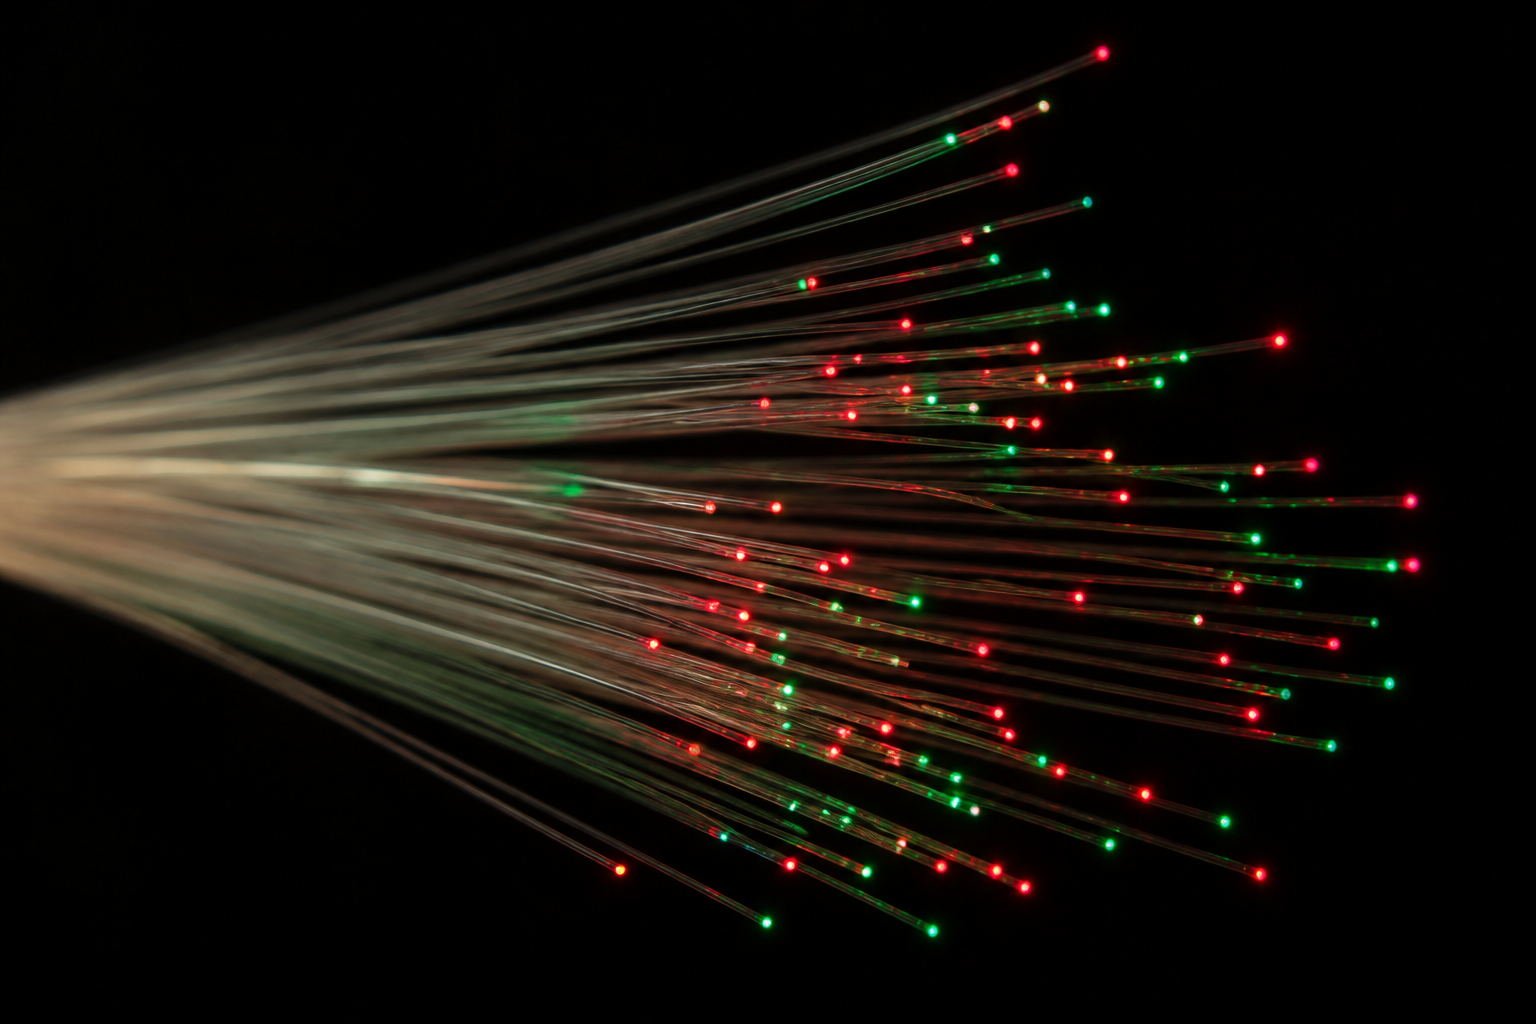
\includegraphics[width=0.58\linewidth]{images/book4/ai/b4-16-optical-fibres-glow.png}

{\small Des \omterm{prop:b2:guided-waves:fibre}{fibres optiques} éclairées par leur extrémité opposée~: une lumière piégée par \omterm{thm:b2:wave-interfaces:snell}{réflexion totale} dans un cœur plus fin qu'un cheveu, et guidée à travers chaque courbe douce.}
\end{omfigure}

\section{Problème~: la cavité du four et la fibre optique}

\begin{problem}[{Problème du week-end --- deux systèmes à ondes guidées présents dans chaque
cuisine et chaque ville~: le four qui cuit avec des ondes stationnaires et
la fibre qui transporte l'internet}]
\label{pb:b2:guided-waves:1}

\medskip
\noindent\textbf{Partie I --- Du magnétron à la cavité.}
Un magnétron injecte \qty{800}{W} à \qty{2.45}{GHz} dans un \omterm{prop:b2:guided-waves:rectangular}{guide d'ondes
rectangulaire} ($a = \qty{8.6}{cm}$, $b = \qty{4.3}{cm}$) qui débouche dans la cavité
du four ($30 \times 30 \times 20$ cm$^3$)~; parois en acier, $\gamma = \qty{1e6}{S/m}$.
\begin{enumerate}
  \item Fréquences de coupure des \omterm{prop:b2:guided-waves:rectangular}{modes TE}$_{10}$, TE$_{20}$, TE$_{01}$ du guide~;
        vérifier que seul TE$_{10}$ se propage à \qty{2.45}{GHz}.
  \item Longueur d'\omterm{prop:b2:guided-waves:plates}{onde guidée}, \omterm{def:b2:dispersion-wave-packets:relation}{vitesses de phase} et de groupe à \qty{2.45}{GHz}.
  \item Amplitude du champ $E_0$ dans le guide pour \qty{800}{W} (formule de puissance
        de TE$_{10}$)~; comparer au champ de claquage de l'air.
  \item Amplitude du \omterm{prop:b2:maxwell-equations:boundary}{courant surfacique} sur la grande face (de l'ordre de
        $E_0/\mu_0c$)~; \omterm{def:b2:dispersion-wave-packets:complex}{épaisseur de peau} et résistance de surface de l'acier~;
        perte par mètre de guide.
  \item Modes de la cavité~: énumérer ceux dont la fréquence est à $3\%$
        de \qty{2.45}{GHz} (essayer $(m, n, p)$ jusqu'à $4$)~; combien~?
  \item Distance entre les points chauds d'un tel mode selon chaque
        axe~; pourquoi le plateau tourne-t-il, et qu'est-ce qu'un «~brasseur de modes~»~?
  \item Le facteur de qualité de la cavité chargée d'aliments vaut environ
        $200$~: largeur de bande de sa réponse~; pourquoi un écart entre la
        fréquence du magnétron et les modes importe peu.
  \item La cavité vide a $Q \approx 3000$~: énergie emmagasinée pour \qty{800}{W}
        injectés, densité d'énergie moyenne, amplitude du champ~; comparer à la
        question 3 et au claquage. Qu'est-ce qui protège le magnétron
        lorsque le four tourne à vide~?
  \item Temps mis par l'énergie pour parcourir les \qty{20}{cm} de guide entre
        le magnétron et la cavité.
  \item Le magnétron est alimenté par un redressement mono-alternance et n'émet
        que pendant une demi-période du secteur~: puissance crête pendant
        les salves pour une moyenne de \qty{800}{W}~; que fait la cavité
        entre les salves (prendre $Q \approx 200$)~?
\end{enumerate}

\medskip
\noindent\textbf{Partie II --- La porte et la coupure.}
\begin{enumerate}[resume]
  \item La grille de la porte a des trous de \qty{1.5}{mm} dans une tôle de \qty{1}{mm}~: longueur
        de décroissance dans un trou et \omterm{def:b2:dispersion-wave-packets:complex}{atténuation} en dB à travers la tôle.
  \item Le bord de la porte est fermé par un «~piège~» quart d'onde~: une cavité
        de profondeur $\lambda/4$ courant autour du cadre, qui présente un circuit
        ouvert au niveau de l'interstice (rappel~: \cref{ch:b2:wave-interfaces})~: profondeur
        de la cavité à \qty{2.45}{GHz}.
  \item La fuite réglementaire vaut \qty{5}{mW/cm^2} à \qty{5}{cm}~: à quelle fraction des
        \qty{800}{W} à travers une porte de \qty{100}{cm^2} cela correspond-il~?
  \item Un conduit de \qty{30}{cm} et de \qty{4}{cm} de diamètre ventile la cavité~: est-il
        sous la coupure à \qty{2.45}{GHz}~? \omterm{def:b2:dispersion-wave-packets:complex}{Atténuation} sur sa longueur.
  \item Pourquoi la grille doit-elle être reliée électriquement au cadre de la porte tout
        autour (à quoi s'apparenterait une rupture de cette liaison)~?
\end{enumerate}

\medskip
\noindent\textbf{Partie III --- La fibre.}
Une fibre à saut d'indice~: cœur $n_1 = 1.465$, gaine $n_2 = 1.460$, diamètre
de cœur \qty{50}{\micro m} (multimode) ou \qty{9}{\micro m} (monomode)~;
$\lambda = \qty{1.55}{\micro m}$~; \omterm{def:b2:dispersion-wave-packets:complex}{atténuation} \qty{0.2}{dB/km}.
\begin{enumerate}[resume]
  \item \omterm{prop:b2:guided-waves:fibre}{Ouverture numérique} et angle d'acceptance~; est-il facile d'y injecter
        la lumière~?
  \item Étalement modal par kilomètre pour la fibre multimode~; débit binaire
        maximal sur \qty{10}{km} (un bit par durée d'étalement).
  \item Nombre de modes de la fibre multimode (admettre $N \approx
        \tfrac12(\pi d\,\mathrm{NA}/\lambda)^2$)~; de la monomode ($d =
        \qty{9}{\micro m}$~: montrer que la même formule donne environ $1$).
  \item Dans la fibre monomode l'étalement restant est chromatique~:
        avec $\omega'' \approx \qty{-0.2}{m^2/s}$ (\cref{ch:b2:dispersion-wave-packets})
        et des impulsions de \qty{50}{ps}, distance sur laquelle une impulsion double~;
        débit binaire sur \qty{100}{km}.
  \item \omterm{def:b2:dispersion-wave-packets:complex}{Atténuation} sur \qty{100}{km} en dB et en rapport de puissances~; \qty{1}{mW}
        en entrée~: puissance de sortie~; avec des amplificateurs tous les \qty{80}{km}, combien
        en faut-il pour une liaison transatlantique de \qty{6000}{km}~?
  \item Fréquence et énergie du photon à \qty{1.55}{\micro m}~; photons par
        seconde dans \qty{1}{mW}, et par bit à \qty{10}{Gbit/s}, à l'entrée
        et après \qty{100}{km}.
  \item Pourquoi \qty{1.55}{\micro m} (penser aux deux mécanismes de perte de la
        silice~: la diffusion Rayleigh, décroissant en $1/\lambda^4$, et l'absorption
        infrarouge croissant au-delà de \qty{1.6}{\micro m})~?
  \item Réflexion de Fresnel au bout clivé d'une fibre face à l'air~: perte en
        dB~; pourquoi les connecteurs utilisent un gel d'adaptation d'indice ou un contact
        physique poli.
  \item Pourquoi une fibre ne rayonne-t-elle pas dans une courbe douce, et pourquoi
        perd-elle de la lumière dans une courbe serrée (penser à l'angle du rayon
        sur la frontière du cœur)~?
  \item Comparer les deux guides de ce problème~: ce qui confine l'onde,
        ce qui limite la bande passante, ce que sont les pertes.
\end{enumerate}
\end{problem}
